%========================================
% MatinBook — Stage 10: Graphics Test
% Version: v1.1
% Purpose:
%   Validate the graphics system of MatinBook v1.1:
%     1. PGFPlots function plots
%     2. Statistical charts (bar, line, scatter)
%     3. Flowcharts with custom TikZ styles
%     4. Trees (binary search tree, expression tree)
%     5. Directed weighted graphs
%     6. 3D surface plots
%     7. Pie charts
%     8. Timelines
%
% Compilation:
%   xelatex -shell-escape stage10-tikz.tex
%   xelatex -shell-escape stage10-tikz.tex
%   (2 passes required for cover + cross-references)
%
% Expected outcome:
%   A professionally typeset PDF demonstrating that every
%   graphics feature renders correctly, with proper Persian
%   captions and working cross-references.
%========================================

%------------------------------------------------------------------------
% Search Path (for tests directory)
%------------------------------------------------------------------------
\makeatletter
\def\input@path{{../}}
\makeatother

%------------------------------------------------------------------------
% Document Class
%------------------------------------------------------------------------
\documentclass{matinbook}

%------------------------------------------------------------------------
% Additional PGFPlots libraries for this test
%------------------------------------------------------------------------
\usepgfplotslibrary{colormaps}

%------------------------------------------------------------------------
% Book Metadata
%------------------------------------------------------------------------
\title{آزمون سیستم گرافیک و نمودارها}
\author{تیم توسعه MatinBook}
\date{مهر ۱۴۰۵}

\booktitle{آزمون سیستم گرافیک و نمودارها}

\renewcommand{\repository}{github.com/matinmahmoudi-cs/matinbook}

%========================================================================
% DOCUMENT
%========================================================================
\begin{document}

%------------------------------------------------------------------------
% FRONT COVER
%------------------------------------------------------------------------
\makecover
    {آزمون سیستم گرافیک و نمودارها}
    {ارزیابی ترسیم، نمودار و دیاگرام در MatinBook}
    {تیم توسعه MatinBook}
    {مهر ۱۴۰۵}

%------------------------------------------------------------------------
% FRONT MATTER (symmetric margins)
%------------------------------------------------------------------------
\frontmatter
\frontmattergeometry

% Title page
\maketitle

% Copyright / Colophon
\thispagestyle{empty}
\vfill
\begin{center}
    {\large\textbf{شناسنامه آزمون}}

    \vspace{0.8cm}

    \begin{tabular}{rl}
        عنوان: & آزمون سیستم گرافیک و نمودارها \\
        نسخه: & \matinbookversion \\
        تاریخ: & \matinbookdate \\
        موتور: & \lr{XeLaTeX} \\
        مجوز: & \lr{MIT} \\
    \end{tabular}

    \vspace{0.8cm}

    {\small این سند بخشی از مجموعه آزمون‌های یکپارچگی \lr{MatinBook} است.}
\end{center}
\clearpage

% Preface
\chapter*{پیشگفتار}
\addcontentsline{toc}{chapter}{پیشگفتار}

این سند، دهمین آزمون از مجموعه‌ی آزمون‌های یکپارچگی
\lr{MatinBook} نسخه‌ی \lr{\matinbookversion} است. هدف آن،
اعتبارسنجی کامل سیستم گرافیک کلاس در هشت حوزه‌ی متمایز
است: نمودار توابع ریاضی، نمودارهای آماری، فلوچارت‌ها،
درخت‌ها، گراف‌ها، نمودارهای سه‌بعدی، نمودارهای دایره‌ای
و خطوط زمانی.

در کتاب‌های فنی و علمی، نمودارها و دیاگرام‌ها نقش محوری
در انتقال مفاهیم پیچیده دارند. یک نمودار حرفه‌ای می‌تواند
جای چند صفحه متن را بگیرد و درک مطلب را چند برابر کند.
\lr{MatinBook} با استفاده از \lr{TikZ}، \lr{PGFPlots} و
\lr{pgf-pie}، این قابلیت‌ها را فراهم می‌سازد.

هر بخش از این آزمون، با مثال‌های عملی و ارجاعات متقابل
همراه است تا خواننده بتواند درستی رفتار هر زیرسیستم را
در بافت واقعی یک کتاب ارزیابی کند.

\clearpage

% Table of Contents
\tableofcontents
\clearpage

% List of Figures
\listoffigures
\clearpage

% List of Tables
\listoftables
\clearpage

%------------------------------------------------------------------------
% MAIN MATTER (wide margin for notes)
%------------------------------------------------------------------------
\mainmatter
\mainmattergeometry

%========================================================================
% CHAPTER 1 — FUNCTION PLOTS
%========================================================================
\chapter{نمودار توابع ریاضی}
\label{chap:function-plots}

\section{مقایسه توابع پایه}
\label{sec:plots-basic}

نمودار \cref{fig:basic-functions} چهار تابع پایه‌ی ریاضی
را مقایسه می‌کند:

\begin{figure}[h]
\centering
\begin{latin}
\begin{tikzpicture}
  \begin{axis}[
    width=\textwidth, height=7cm,
    xlabel={$x$},
    ylabel={$f(x)$},
    title={Comparison of Common Mathematical Functions},
    grid=major,
    legend pos=north west,
    domain=-3:3,
    samples=200,
    xmin=-3, xmax=3,
    ymin=-5, ymax=10
  ]
    \addplot[matinblue, thick] {x^2};
    \addlegendentry{$x^2$}

    \addplot[matinred, thick] {x^3};
    \addlegendentry{$x^3$}

    \addplot[matinorange, thick] {exp(x)};
    \addlegendentry{$e^x$}

    \addplot[matingreen, thick, domain=0:3] {sqrt(x)};
    \addlegendentry{$\sqrt{x}$}
  \end{axis}
\end{tikzpicture}
\end{latin}
\caption{مقایسه توابع $x^{2}$، $x^{3}$، $e^{x}$ و $\sqrt{x}$}
\label{fig:basic-functions}
\end{figure}

\mnote{نمودارها با \lr{PGFPlots} رسم می‌شوند و از پالت رنگی \lr{MatinBook} پیروی می‌کنند.}

\section{توابع مثلثاتی}
\label{sec:plots-trig}

نمودار \cref{fig:trig-functions} توابع مثلثاتی اصلی را
نشان می‌دهد:

\begin{figure}[h]
\centering
\begin{latin}
\begin{tikzpicture}
  \begin{axis}[
    width=\textwidth, height=6.5cm,
    xlabel={$x$},
    ylabel={$f(x)$},
    title={Trigonometric Functions},
    grid=major,
    legend pos=north west,
    domain=-2*pi:2*pi,
    samples=300,
    xtick={-2*pi, -1.5*pi, -pi, -0.5*pi, 0, 0.5*pi, pi, 1.5*pi, 2*pi},
    xticklabels={$-2\pi$, $-\frac{3\pi}{2}$, $-\pi$, $-\frac{\pi}{2}$,
                 $0$, $\frac{\pi}{2}$, $\pi$, $\frac{3\pi}{2}$, $2\pi$},
    ymin=-1.5, ymax=1.5
  ]
    \addplot[matinblue, thick] {sin(deg(x))};
    \addlegendentry{$\sin x$}

    \addplot[matinred, thick] {cos(deg(x))};
    \addlegendentry{$\cos x$}

    \addplot[matinorange, thick, dashed, restrict y to domain=-3:3] {tan(deg(x))};
    \addlegendentry{$\tan x$}
  \end{axis}
\end{tikzpicture}
\end{latin}
\caption{توابع مثلثاتی $\sin x$، $\cos x$ و $\tan x$}
\label{fig:trig-functions}
\end{figure}

\section{توابع فعال‌سازی}
\label{sec:plots-activation}

نمودار \cref{fig:activation-functions} توابع فعال‌سازی
رایج در شبکه‌های عصبی را نشان می‌دهد:

\begin{figure}[h]
\centering
\begin{latin}
\begin{tikzpicture}
  \begin{axis}[
    width=\textwidth, height=6.5cm,
    xlabel={$x$},
    ylabel={$y$},
    title={Activation Functions},
    grid=major,
    legend pos=north west,
    domain=-5:5,
    samples=200
  ]
    \addplot[matinblue, ultra thick] {1/(1+exp(-x))};
    \addlegendentry{$\sigma(x) = \frac{1}{1+e^{-x}}$}

    \addplot[matinpurple, thick, dashed] {tanh(x)};
    \addlegendentry{$\tanh x$}

    \addplot[matinorange, thick, dotted] {max(0, x)};
    \addlegendentry{$\max(0, x)$}
  \end{axis}
\end{tikzpicture}
\end{latin}
\caption{توابع فعال‌سازی در شبکه‌های عصبی}
\label{fig:activation-functions}
\end{figure}

%========================================================================
% CHAPTER 2 — STATISTICAL CHARTS
%========================================================================
\chapter{نمودارهای آماری}
\label{chap:statistical-charts}

\section{نمودار میله‌ای}
\label{sec:charts-bar}

نمودار \cref{fig:language-popularity} محبوبیت زبان‌های
برنامه‌نویسی را نشان می‌دهد:

\begin{figure}[h]
\centering
\begin{latin}
\begin{tikzpicture}
  \begin{axis}[
    width=\textwidth, height=6.5cm,
    ybar,
    symbolic x coords={Python, JavaScript, Java, C++, Go, Rust, TypeScript},
    xtick=data,
    ylabel={Popularity (\%)},
    title={Programming Language Popularity - 2025},
    grid=major,
    bar width=18pt,
    ymin=0, ymax=35,
    nodes near coords,
    nodes near coords align={vertical},
    every node near coord/.append style={font=\small}
  ]
    \addplot[fill=matinblue!70] coordinates {
      (Python, 30)
      (JavaScript, 24)
      (Java, 17)
      (C++, 12)
      (Go, 8)
      (Rust, 5)
      (TypeScript, 4)
    };
  \end{axis}
\end{tikzpicture}
\end{latin}
\caption{محبوبیت زبان‌های برنامه‌نویسی در سال ۲۰۲۵}
\label{fig:language-popularity}
\end{figure}

\section{نمودار خطی مقایسه‌ای}
\label{sec:charts-line}

نمودار \cref{fig:complexity-comparison} رشد پیچیدگی
الگوریتم‌ها را با افزایش اندازه‌ی ورودی نشان می‌دهد:

\begin{figure}[h]
\centering
\begin{latin}
\begin{tikzpicture}
  \begin{axis}[
    width=\textwidth, height=6.5cm,
    xlabel={Input Size ($n$)},
    ylabel={Operations},
    title={Algorithm Complexity Comparison},
    grid=major,
    legend pos=north west,
    domain=0:50,
    samples=100,
    ymin=0, ymax=3000
  ]
    \addplot[matinred, thick] {x^2};
    \addlegendentry{$O(n^2)$}

    \addplot[matinorange, thick] {x*ln(x)};
    \addlegendentry{$O(n \log n)$}

    \addplot[matinblue, thick] {x};
    \addlegendentry{$O(n)$}

    \addplot[matingreen, thick] {10*ln(x)};
    \addlegendentry{$O(\log n)$}
  \end{axis}
\end{tikzpicture}
\end{latin}
\caption{مقایسه رشد پیچیدگی الگوریتم‌ها}
\label{fig:complexity-comparison}
\end{figure}

\section{نمودار پراکندگی}
\label{sec:charts-scatter}

نمودار \cref{fig:scatter-plot} رابطه‌ی میان ساعت مطالعه
و نمره‌ی امتحان را نشان می‌دهد:

\begin{figure}[h]
\centering
\begin{latin}
\begin{tikzpicture}
  \begin{axis}[
    width=\textwidth, height=6cm,
    xlabel={Hours Studied},
    ylabel={Exam Score},
    title={Study Time vs. Exam Performance},
    grid=major,
    legend pos=south east
  ]
    \addplot[only marks, mark=*, color=matinblue, mark size=2pt] coordinates {
      (1, 45) (2, 52) (3, 58) (4, 65) (5, 70)
      (6, 75) (7, 80) (8, 85) (9, 88) (10, 92)
      (1.5, 48) (2.5, 55) (3.5, 62) (4.5, 68) (5.5, 73)
      (6.5, 78) (7.5, 82) (8.5, 86) (9.5, 90)
    };
    \addlegendentry{Data points}

    \addplot[matinred, thick, domain=0:11] {5*x + 40};
    \addlegendentry{Regression line}
  \end{axis}
\end{tikzpicture}
\end{latin}
\caption{نمودار پراکندگی با خط رگرسیون}
\label{fig:scatter-plot}
\end{figure}

%========================================================================
% CHAPTER 3 — FLOWCHARTS AND DIAGRAMS
%========================================================================
\chapter{فلوچارت‌ها و دیاگرام‌ها}
\label{chap:flowcharts}

\section{فلوچارت تصمیم‌گیری}
\label{sec:flowcharts-decision}

فلوچارت \cref{fig:flowchart} فرآیند اعتبارسنجی و پردازش
داده را نشان می‌دهد:

\begin{figure}[h]
\centering
\begin{latin}
\begin{tikzpicture}[
  node distance=2cm,
  scale=0.95,
  transform shape,
  arrow/.style={thick,->,>=stealth}
]
  \node[block] (start) {Start};
  \node[block, below of=start] (input) {Read Input Data};
  \node[decision, below of=input] (validate) {Data Valid?};
  \node[block, right of=validate, xshift=3.5cm] (process) {Process Data};
  \node[block, below of=validate, yshift=-1.5cm] (error) {Show Error Message};
  \node[block, below of=process] (output) {Generate Output};
  \node[block, below of=output] (save) {Save Results};
  \node[block, below of=save] (end) {End};

  \draw[arrow] (start) -- (input);
  \draw[arrow] (input) -- (validate);
  \draw[arrow] (validate) -- node[anchor=south] {Yes} (process);
  \draw[arrow] (validate) -- node[anchor=east] {No} (error);
  \draw[arrow] (process) -- (output);
  \draw[arrow] (output) -- (save);
  \draw[arrow] (save) -- (end);
  \draw[arrow] (error) -- ++(-3.5,0) |- (input);
\end{tikzpicture}
\end{latin}
\caption{فلوچارت اعتبارسنجی و پردازش داده}
\label{fig:flowchart}
\end{figure}

\section{دیاگرام معماری نرم‌افزار}
\label{sec:flowcharts-architecture}

دیاگرام \cref{fig:architecture} معماری یک برنامه‌ی وب
مدرن را نشان می‌دهد:

\begin{figure}[h]
\centering
\begin{latin}
\begin{tikzpicture}[
  node distance=2.5cm,
  scale=0.85,
  transform shape,
  arrow/.style={thick,<->,>=stealth},
  component/.style={rectangle, draw=matindarkblue, fill=matinlightblue!30,
                    text width=3.5cm, text centered, rounded corners,
                    minimum height=2cm, font=\small}
]
  \node[component] (frontend) {Frontend\\React / Vue};
  \node[component, right of=frontend, xshift=3cm] (api) {REST API\\Express / FastAPI};
  \node[component, right of=api, xshift=3cm] (database) {Database\\PostgreSQL};

  \node[component, below of=api, yshift=-1.5cm] (cache) {Cache\\Redis};
  \node[component, left of=cache, xshift=-1.5cm] (queue) {Queue\\RabbitMQ};
  \node[component, right of=cache, xshift=1.5cm] (storage) {Storage\\S3 / MinIO};

  \draw[arrow] (frontend) -- (api);
  \draw[arrow] (api) -- (database);
  \draw[arrow] (api) -- (cache);
  \draw[arrow] (api) -- (queue);
  \draw[arrow] (api) -- (storage);
\end{tikzpicture}
\end{latin}
\caption{معماری یک برنامه وب مدرن}
\label{fig:architecture}
\end{figure}

%========================================================================
% CHAPTER 4 — TREES AND GRAPHS
%========================================================================
\chapter{درخت‌ها و گراف‌ها}
\label{chap:trees-graphs}

\section{درخت جستجوی دودویی (BST)}
\label{sec:trees-bst}

درخت \cref{fig:bst} یک درخت جستجوی دودویی را نشان
می‌دهد:

\begin{figure}[h]
\centering
\begin{latin}
\begin{tikzpicture}[
  scale=0.9,
  transform shape,
  level distance=2cm,
  level 1/.style={sibling distance=5cm},
  level 2/.style={sibling distance=2.5cm},
  level 3/.style={sibling distance=1.5cm}
]
  \node[treenode] {50}
    child {node[treenode] {30}
      child {node[treenode] {20}}
      child {node[treenode] {40}
        child {node[treenode] {35}}
        child {node[treenode] {45}}
      }
    }
    child {node[treenode] {70}
      child {node[treenode] {60}}
      child {node[treenode] {80}
        child {node[treenode] {75}}
        child[missing]
      }
    };
\end{tikzpicture}
\end{latin}
\caption{درخت جستجوی دودویی (\lr{Binary Search Tree})}
\label{fig:bst}
\end{figure}

\section{درخت بیان ریاضی}
\label{sec:trees-expression}

درخت \cref{fig:expression-tree} بیان ریاضی
$3x + (5 - 2)$ را نشان می‌دهد:

\begin{figure}[h]
\centering
\begin{latin}
\begin{tikzpicture}[
  level distance=1.8cm,
  level 1/.style={sibling distance=4cm},
  level 2/.style={sibling distance=2cm},
  opnode/.style={circle, draw=matinorange, fill=matinlightorange!30, minimum size=0.8cm},
  numnode/.style={circle, draw=matinblue, fill=matinlightblue!30, minimum size=0.8cm}
]
  \node[opnode] {$+$}
    child {node[opnode] {$\times$}
      child {node[numnode] {$3$}}
      child {node[numnode] {$x$}}
    }
    child {node[opnode] {$-$}
      child {node[numnode] {$5$}}
      child {node[numnode] {$2$}}
    };
\end{tikzpicture}
\end{latin}
\caption{درخت بیان ریاضی $3x + (5 - 2)$}
\label{fig:expression-tree}
\end{figure}

\section{گراف جهت‌دار وزن‌دار}
\label{sec:trees-graph}

گراف \cref{fig:directed-graph} یک گراف جهت‌دار وزن‌دار
با پنج رأس را نشان می‌دهد:

\begin{figure}[h]
\centering
\begin{latin}
\begin{tikzpicture}[
  node distance=2.5cm,
  vertex/.style={circle, draw=matindarkblue, fill=matinlightblue!30,
                 minimum size=1cm, font=\bfseries},
  edge/.style={thick,->,>=stealth}
]
  \node[vertex] (A) at (0,0) {A};
  \node[vertex] (B) at (3,2) {B};
  \node[vertex] (C) at (6,0) {C};
  \node[vertex] (D) at (3,-2) {D};
  \node[vertex] (E) at (1.5,-3.5) {E};

  \draw[edge] (A) -- node[anchor=south] {5} (B);
  \draw[edge] (B) -- node[anchor=south] {3} (C);
  \draw[edge] (C) -- node[anchor=west] {4} (D);
  \draw[edge] (D) -- node[anchor=north] {2} (A);
  \draw[edge] (A) -- node[anchor=east] {7} (E);
  \draw[edge] (D) -- node[anchor=east] {6} (E);
  \draw[edge] (B) to[bend left] node[anchor=west] {8} (D);
\end{tikzpicture}
\end{latin}
\caption{گراف وزن‌دار جهت‌دار با ۵ رأس}
\label{fig:directed-graph}
\end{figure}

%========================================================================
% CHAPTER 5 — ADVANCED TIKZ
%========================================================================
\chapter{نمودارهای پیشرفته}
\label{chap:advanced-tikz}

\section{نمودار سه‌بعدی}
\label{sec:advanced-3d}

نمودار \cref{fig:3d-surface} یک سطح سه‌بعدی را نشان
می‌دهد:

\begin{figure}[h]
\centering
\begin{latin}
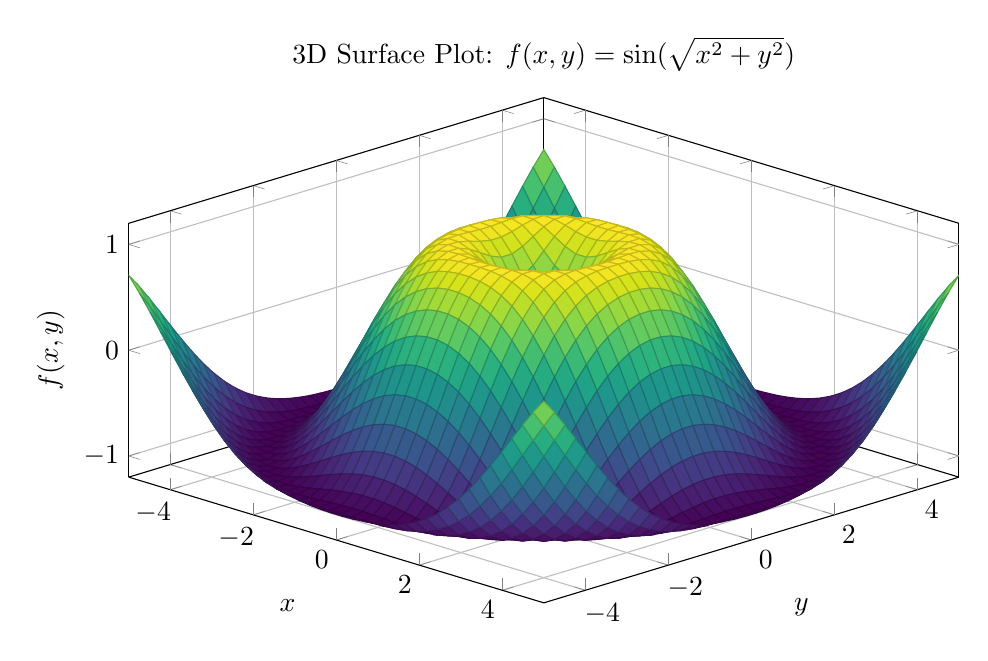
\begin{tikzpicture}
  \begin{axis}[
    width=\textwidth, height=8cm,
    xlabel={$x$},
    ylabel={$y$},
    zlabel={$f(x,y)$},
    title={3D Surface Plot: $f(x,y) = \sin(\sqrt{x^2+y^2})$},
    view={45}{35},
    grid=major
  ]
    \addplot3[
      surf,
      domain=-5:5,
      domain y=-5:5,
      samples=40,
      samples y=40,
      colormap/viridis
    ] {sin(deg(sqrt(x^2+y^2)))};
  \end{axis}
\end{tikzpicture}
\end{latin}
\caption{نمودار سه‌بعدی تابع $f(x,y) = \sin(\sqrt{x^{2}+y^{2}})$}
\label{fig:3d-surface}
\end{figure}

\section{نمودار دایره‌ای}
\label{sec:advanced-pie}

نمودار \cref{fig:pie-chart} توزیع استفاده از زبان‌های
برنامه‌نویسی را نشان می‌دهد:

\begin{figure}[h]
\centering
\begin{latin}
\begin{tikzpicture}
  \pie[
    radius=3,
    text=legend,
    color={matinblue, matingreen, matinorange, matinred, matinpurple}
  ]{
    35/Python,
    25/JavaScript,
    20/Java,
    12/C++,
    8/Other
  }
\end{tikzpicture}
\end{latin}
\caption{توزیع استفاده از زبان‌های برنامه‌نویسی}
\label{fig:pie-chart}
\end{figure}

\section{خط زمانی}
\label{sec:advanced-timeline}

خط زمانی \cref{fig:timeline} تاریخچه‌ی زبان‌های
برنامه‌نویسی را نشان می‌دهد:

\begin{figure}[h]
\centering
\begin{latin}
\begin{tikzpicture}[
  xscale=0.7,
  timeline/.style={thick,->,>=stealth},
  event/.style={rectangle, draw=matindarkblue, fill=matinlightblue!30,
                text width=2.2cm, text centered, rounded corners,
                minimum height=1cm, inner sep=3pt, font=\footnotesize},
  arrow/.style={thick,->,>=stealth}
]
  \draw[timeline] (0,0) -- (14,0);

  \foreach \x/\year in {0/1990, 3.5/2000, 7/2010, 10.5/2020, 14/2025} {
    \draw[thick] (\x,-0.2) -- (\x,0.2);
    \node[below] at (\x,-0.3) {\small\year};
  }

  \node[event, above] at (0,1.2) {Python\\Created};
  \node[event, above] at (3.5,1.2) {C\#\\Released};
  \node[event, above] at (7,1.2) {Rust\\First Stable};
  \node[event, below] at (7,-1.2) {Go\\Released};
  \node[event, above] at (10.5,1.2) {TypeScript\\Released};
  \node[event, below] at (14,-1.2) {AI/ML\\Boom};

  \draw[arrow] (0,0.3) -- (0,0.5);
  \draw[arrow] (3.5,0.3) -- (3.5,0.5);
  \draw[arrow] (7,0.3) -- (7,0.5);
  \draw[arrow] (7,-0.3) -- (7,-0.5);
  \draw[arrow] (10.5,0.3) -- (10.5,0.5);
  \draw[arrow] (14,-0.3) -- (14,-0.5);
\end{tikzpicture}
\end{latin}
\caption{خط زمانی تاریخچه زبان‌های برنامه‌نویسی}
\label{fig:timeline}
\end{figure}

%========================================================================
% CHAPTER 6 — SUMMARY
%========================================================================
\chapter{خلاصه‌ی نتایج}
\label{chap:summary}

\section{وضعیت سیستم گرافیک}
\label{sec:summary-status}

جدول \cref{tab:graphics-status} وضعیت قابلیت‌های گرافیکی
\lr{MatinBook} را نشان می‌دهد.

\begin{matintable}{وضعیت قابلیت‌های گرافیکی}{tab:graphics-status}
\begin{tblr}{
    width = \textwidth,
    colspec = {l X[c] X[c]},
    hlines, vlines,
    colsep = 8pt,
    rowsep = 4pt,
    row{1} = {font=\bfseries},
}
نوع نمودار & موارد آزمایش‌شده & وضعیت \\
توابع ریاضی & ۳ نمودار (پایه، مثلثاتی، فعال‌سازی) & \textcolor{matingreen}{فعال} \\
نمودار آماری & میله‌ای، خطی، پراکندگی & \textcolor{matingreen}{فعال} \\
فلوچارت & اعتبارسنجی داده + معماری نرم‌افزار & \textcolor{matingreen}{فعال} \\
درخت & \lr{BST} + درخت بیان ریاضی & \textcolor{matingreen}{فعال} \\
گراف & گراف وزن‌دار جهت‌دار & \textcolor{matingreen}{فعال} \\
سه‌بعدی & نمودار سطح \lr{3D} & \textcolor{matingreen}{فعال} \\
دایره‌ای & نمودار \lr{Pie Chart} & \textcolor{matingreen}{فعال} \\
خط زمانی & تاریخچه زبان‌های برنامه‌نویسی & \textcolor{matingreen}{فعال} \\
\end{tblr}
\end{matintable}

\section{معیارهای ارزیابی}
\label{sec:summary-criteria}

در این آزمون، سیستم گرافیک \lr{MatinBook} بر اساس پنج
معیار ارزیابی شد:

\begin{enumerate}
    \item \textbf{کیفیت ترسیم}: دقت و زیبایی نمودارها.
    \item \textbf{رنگ‌آمیزی}: هماهنگی با پالت \lr{MatinBook}.
    \item \textbf{کپشن فارسی}: متن‌های گویا و ارجاع‌پذیر.
    \item \textbf{تنوع}: پوشش انواع رایج نمودار.
    \item \textbf{پایداری}: رفتار یکنواخت در همه‌ی نمودارها.
\end{enumerate}

\section{نتیجه‌گیری}
\label{sec:summary-conclusion}

\textbf{تمام زیرسیستم‌های گرافیک \lr{MatinBook} نسخه‌ی
\lr{\matinbookversion} با موفقیت بارگذاری و آزمایش شدند.
دوازده نمودار مختلف شامل توابع ریاضی، نمودارهای آماری،
فلوچارت، درخت، گراف، نمودار سه‌بعدی، نمودار دایره‌ای
و خط زمانی، همگی به‌درستی رسم می‌شوند.}

%------------------------------------------------------------------------
% BACK MATTER (symmetric margins)
%------------------------------------------------------------------------
\backmatter
\frontmattergeometry

% Bibliography (empty placeholder)
\printbibliography[title={منابع و مراجع}]

% Index
\printindex

%------------------------------------------------------------------------
% BACK COVER
%------------------------------------------------------------------------
\authorbio{%
    تیم توسعه‌ی \lr{MatinBook}، گروهی از پژوهشگران و برنامه‌نویسان
    فارسی‌زبان است که با هدف ارائه‌ی یک راه‌حل حرفه‌ای برای
    حروف‌چینی کتاب‌های فنی فارسی فعالیت می‌کند. این پروژه حاصل
    سال‌ها تجربه در حوزه‌ی نشر دیجیتال و برنامه‌نویسی است.
}

\makebackcover{%
    این سند، دهمین آزمون از مجموعه‌ی آزمون‌های یکپارچگی
    \lr{MatinBook} نسخه‌ی \lr{\matinbookversion} است.

    \vspace{0.5cm}

    \textbf{زیرسیستم‌های آزموده‌شده:}
    \begin{itemize}
        \item نمودار توابع ریاضی
        \item نمودارهای آماری
        \item فلوچارت‌ها
        \item درخت‌ها
        \item گراف‌ها
        \item نمودار سه‌بعدی
        \item نمودار دایره‌ای
        \item خط زمانی
    \end{itemize}
}

\end{document}